\documentclass{beamer}
\usepackage{color}
\usepackage{hyperref}
% \usepackage{pgf, pgfarrows, pgfnodes}
\usepackage{mathtools}
\usetheme{AnnArbor}
\title[https://github.com/cheraaqee/popSR]{Perceptually-Optimized Loss Function for Image Super-Resolution}
\author[ICSPIS2021]{\small Amirhossein Arezoomand \inst{1} \and Pooryaa Cheraaqee \inst{1} \and Azadeh Mansouri \inst{1}}
\institute[]{\inst{1} \textbf{Department of\\ Electrical and Computer Engineering,\\ Kharazmi University}}
% \date{\today}
\begin{document}
%%%%
\begin{frame}
\frametitle{ICSPIS 2021}
\titlepage
\end{frame}
%%%%
\section*{Outline}
\begin{frame}
\frametitle{Outline}
\tableofcontents[pausesections]
\end{frame}
%%%
\section{Problem Definition}
\tableofcontents[currentsection]
\subsection{Image Super-Resolution}
\begin{frame}
\frametitle{What is \emph{Super-Resolution}?}
\begin{itemize}
\visible<1->{
\item \textbf{increasing the dimension}}
\begin{itemize}
\visible<2,3>{
\item $\text{input (}X_{M\times N}) \xrightarrow{\text{upsampling by a factor of 2 (i.e. }2\uparrow)} \text{output (}Y_{2M\times 2N})$}
\visible<3>{
\item BiLinear, Bicubic, etc.}
\end{itemize}
\visible<4->{
\item
\textcolor{red}{\textbf{!! Preserving the quality !!}}}
\end{itemize}
\visible<5->{
\begin{center}
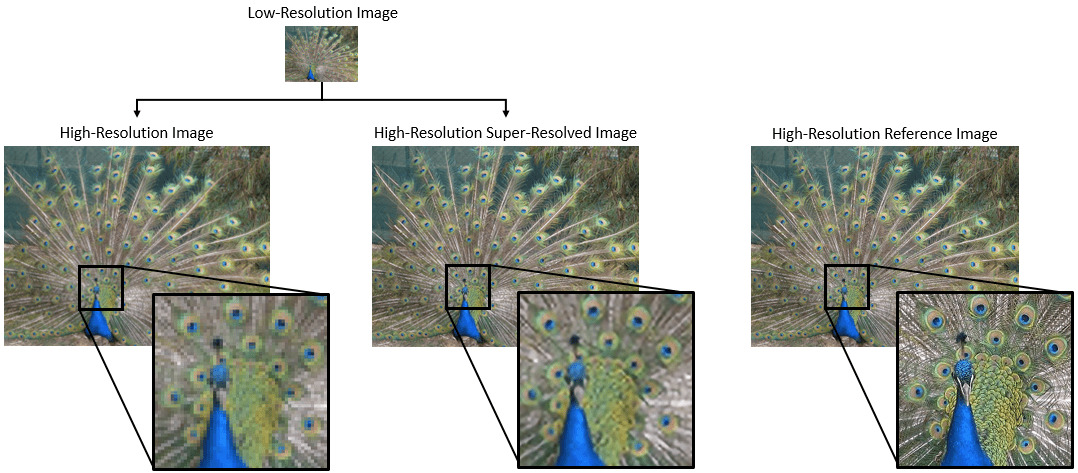
\includegraphics[height=4cm]{sr_sample}
\end{center}
}
\end{frame}
\subsection{Loss Function}
\begin{frame}
\frametitle{CNNs and Loss Functions}
\begin{itemize}
\visible<1->{
\item Super-Resolver CNNs
}
\end{itemize}

\end{frame}
%%%
\section{Previous Attempts}
%%%
\section{Our Approach}
%%%
\section{Results}
\subsection{Quantitative}
\subsection{Qualitative}
%%%%
\section{Conclusion\& Future Works}
\end{document}
